%%%%%%%%%%%%%%%%%%%%%%%%%%%%%%%%%%%%%%%%%
% Homework Assignment Article
% LaTeX Template
% Version 1.3.1 (ECL) (08/08/17)
%
% This template has been downloaded from:
% Overleaf
%
% Original author:
% Victor Zimmermann (zimmermann@cl.uni-heidelberg.de)
%
% License:
% CC BY-SA 4.0 (https://creativecommons.org/licenses/by-sa/4.0/)
%
%%%%%%%%%%%%%%%%%%%%%%%%%%%%%%%%%%%%%%%%%

%----------------------------------------------------------------------------------------

\documentclass[a4paper]{article} % Uses article class in A4 format

%----------------------------------------------------------------------------------------
%	FORMATTING
%----------------------------------------------------------------------------------------

\addtolength{\hoffset}{-2.25cm}
\addtolength{\textwidth}{4.5cm}
\addtolength{\voffset}{-3.25cm}
\addtolength{\textheight}{5cm}
\setlength{\parskip}{0pt}
\setlength{\parindent}{0in}

%----------------------------------------------------------------------------------------
%	PACKAGES AND OTHER DOCUMENT CONFIGURATIONS
%----------------------------------------------------------------------------------------

\usepackage{blindtext} % Package to generate dummy text
% \usepackage[style=numeric,sorting=none]{biblatex}
\usepackage{charter} % Use the Charter font
\usepackage[utf8]{inputenc} % Use UTF-8 encoding
\usepackage{microtype} % Slightly tweak font spacing for aesthetics

\usepackage[english]{babel} % Language hyphenation and typographical rules

\usepackage{amsthm, amsmath, amssymb} % Mathematical typesetting
\usepackage{float} % Improved interface for floating objects
\usepackage[final, colorlinks = true, 
            linkcolor = black, 
            citecolor = black]{hyperref} % For hyperlinks in the PDF
\usepackage{graphicx, multicol} % Enhanced support for graphics
\usepackage{xcolor} % Driver-independent color extensions
\usepackage{marvosym, wasysym} % More symbols
\usepackage{rotating} % Rotation tools
\usepackage{censor} % Facilities for controlling restricted text
\usepackage{listings, style/lstlisting} % Environment for non-formatted code, !uses style file!
\usepackage{color}

\definecolor{dkgreen}{rgb}{0,0.6,0}
\definecolor{gray}{rgb}{0.5,0.5,0.5}
\definecolor{mauve}{rgb}{0.58,0,0.82}
\lstset{frame=tb,
  language=Java,
  aboveskip=3mm,
  belowskip=3mm,
  showstringspaces=false,
  columns=flexible,
  basicstyle={\small\ttfamily},
  numbers=none,
  numberstyle=\tiny\color{gray},
  keywordstyle=\color{blue},
  commentstyle=\color{dkgreen},
  stringstyle=\color{mauve},
  breaklines=true,
  breakatwhitespace=true,
  tabsize=3
}
\usepackage{pseudocode} % Environment for specifying algorithms in a natural way
\usepackage{style/avm} % Environment for f-structures, !uses style file!
\usepackage{booktabs} % Enhances quality of tables

\usepackage{tikz-qtree} % Easy tree drawing tool
\tikzset{every tree node/.style={align=center,anchor=north},
         level distance=2cm} % Configuration for q-trees
\usepackage{style/btree} % Configuration for b-trees and b+-trees, !uses style file!

% \usepackage[backend=biber,style=numeric,
            % sorting=nyt]{biblatex} % Complete reimplementation of bibliographic facilities
% \addbibresource{ecl.bib}
\usepackage{csquotes} % Context sensitive quotation facilities

\usepackage[yyyymmdd]{datetime} % Uses YEAR-MONTH-DAY format for dates
\renewcommand{\dateseparator}{-} % Sets dateseparator to '-'

\usepackage{fancyhdr} % Headers and footers
\pagestyle{fancy} % All pages have headers and footers
\fancyhead{}\renewcommand{\headrulewidth}{0pt} % Blank out the default header
\fancyfoot[L]{School of Computing, Macquarie University} % Custom footer text
\fancyfoot[C]{} % Custom footer text
\fancyfoot[R]{\thepage} % Custom footer text

\usepackage{comment}
\newcommand{\note}[1]{\marginpar{\scriptsize \textcolor{red}{#1}}} % Enables comments in red on margin

\hypersetup{
    colorlinks=true,
    linkcolor=blue,
    filecolor=magenta,      
    urlcolor=cyan,
    pdftitle={COMP3100 Stage 1 Report},
    pdfpagemode=FullScreen,
    }

%----------------------------------------------------------------------------------------

\begin{document}

%----------------------------------------------------------------------------------------
%	TITLE SECTION
%----------------------------------------------------------------------------------------

\title{COMP3100 project report} % Article title
\fancyhead[C]{}
\hrule \medskip % Upper rule
\begin{minipage}{1\textwidth} % Center of title section
\centering 
\large % Title text size
Project report: Stage 2\\ % Assignment title and number
COMP3100 Distributed Systems, S2, 2022\\
\normalsize % Subtitle text size
SID: 45456070, Name: Beau Williams
%%%%\\ % Assignment subtitle
\end{minipage}
\medskip\hrule % Lower rule
\bigskip

%----------------------------------------------------------------------------------------
%	ARTICLE CONTENTS
%----------------------------------------------------------------------------------------

\section*{1. Introduction}
For this COMP3100 assignment we will discuss the process of designing and implementing a new job scheduling algorithm for the Distributed Systems Server Simulator (DSSIM)\cite{dssim}. This report shall cover stage 2 of this assignment, which involves the implementation of the a new Scheduler Algorithm, which will be called First Available Capable Scheduler (FAC), as well as interfacing with the DSSIM to perform simulations with provided test criteria to determine the performance of this new algorithm.
\newline

The purpose of the report coupled with the design and implementation of the FAC Scheduler is intended to test our understanding of Distributed System in relation to the performance tradeoffs of verious scheduling algorithms. It will be made clear that there is no silver bullet algorithm that will perform more efficiently in every aspect (cost, turnaround time, utilisation). As a result, in order to design an effective algorithm one must make a choice as to which aspect of performance they wish to optimise for. Design complexity is not inherently a solution to this optimisation dilemma either. By simply adding more features to an algorithm not only does its characteristics change, but also it often becomes harder to maintain. While there might be some optimisations that inch out slightly better algorithm performance in all aspects, it's still not fundamentally a better design, given that it is still the basic implementation but with some added optimisations. As the old saying goes, less is often more. The design of the FAC scheduler is purposefully simple, albeit at the cost of a slightly higher operating cost (and design complexity), however it does improve the turnaround time which is the very goal of this implementation.
\newline


\section*{2. FAC Scheduler Overview}

At a high level, the job scheduling system that we are creating adopts a similar approach to the Largest Round Robin (LRR) and First Fit (FF) algorithms. It has been designed to blend the turnaround time efficiency of FF algorithms and the utilisation efficiency of the LRR algorithm to create an algorithm the exhibits greater turnaround time efficiency over the baseline algorithms First Fit, Best Fit, Worst Fit and First Capable.
\newline

\section*{3. Problem Definition}

Here we discuss the problem that the First Available Capable algorithm seeks to solve, namely we wish to optimise for turnaround time, while not significantly increasing rental cost and decreasing resource utilisation efficiency.
\newline

This problem can be described as the optimisation trilemma that is made up of a combination of the three hey performance characteristics of a scheduling algorithm. Namely, rental cost, resource utilisation and turnaround time.
\newline

At best a scheduling algorithm designer can pick two characteristics to optimise for, at the expense of the third not chosen characteristic. It is evident that there is a direct correlation to performance improvements to one characteristic, which shall negatively affect the performance of another characteristic.  


\section*{4. Algorithm Description}

First Avaailable Capable Scheduler is designed to improve upon the baseline algorithm First Fit by combining Largest Round Robin as a fall back scheduler when there are no available servers. The key difference between First Fit and First Available Capable is that FAC is designed to evenly distribute jobs to busy servers when there are non available, explicitly preferring larger server types.

In regards to the problem description, it has been chosen to improve the turnaround time of this algorithm, while not causing a significant detriment to the other two remaining characteristics, rental cost and resource utilisation.

\subsection*{4.1. Last Round Robin}

Last Round Robin (LRR) is designed to dispatch jobs to the largest servers available. It determines the largest servers by their core count, and distributes jobs evenly to those servers in a round robin fashion. Initially it will begin with the first server located from the get servers result returned from the DSSIM. Once the first job has been dispatched it will then proceed to increment a counter, dispatching jobs to each server one by one until it reaches the last server. At this point it will start from the first server and repeat this cycle until there are no more remaining jobs to dispatch. This method exhibits moderately efficient resource utilisation and turnaround time are the expense of rental cost.

\subsection*{4.2. First Fit}

First Fit (FF) is an algorithm that is designed to dispatch jobs to the first available server, that is also capable or running the job. It works of a simple assumption that if a job was dispatched to a server it will no longer be available (likely) to receive a job when dispatching the next job. This simple design means that first fit constantly targets the first server it finds that is available. Once available servers are exhausted, it will simply dispatch jobs to the first server it finds. FF is a simple implementation that has low code complexity. It has an optimised turnaround time but this comes at the detriment of rental cost and resource utilisation. It can be noted that first fit under performs in scenarios where there are no available servers are compared to LRR.

\subsection*{4.2. First Available Capable}

First Available Capable (FAC) is designed to be an elegant algorithm that is a hybrid of LRR and FF. Given that the problem definition states that we wish to maximise for turnaround time efficiency, we choose to improve upon the FF algorithm which has the greatest turnaround time efficiency of the baseline algorithms (FF, WF, BF and FC). FAC works by storing a list of capable servers upon first run on the client side. This list is used as the fallback list where jobs are distributed to capable servers in a similar fashion to LRR. When servers are available to receive jobs FAC simply sends it to the first available server. When servers are not available, FAC is explicitly designed to evenly distribute jobs to the largest capable (busy) servers. This fallback technique ensures that for situations where there are a large amount of jobs and few servers, that the turnaround time performance is optimised. In scenarios where there are many servers available, FAC exhibits similar characteristics to FF in that it has an optimised turnaround time efficiency.
\newline

The FAC Scheduler Algorithm is shown at a high level by figure \ref{DSSIM}
\begin{figure}[H]
    \centering
    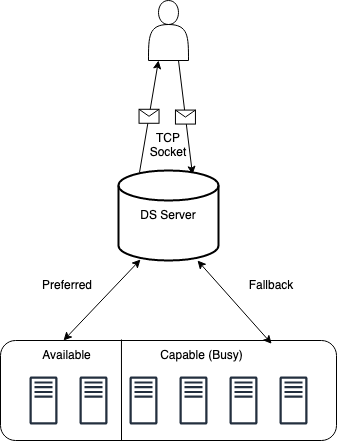
\includegraphics[scale=0.4]{images/fac.png}
    \caption{FAC Scheduler Architecture}
    \label{DSSIM}
\end{figure}


\section*{5. Implementation}
The implementation of the FAC Scheduling algorithm is designed to use minimal dependencies. Preferring to use well utilised data structures available in the standard Java library such as a Arraylists. A while loop is used for simplicity over a for loop to implement the core logic of the algorithm.

\subsection*{5.1. Tooling}
This algorithm was programmed using a modal text editor called neovim\cite{neovim}, coupled with the the Ecplipse Language Server for Java (LSP)\cite{lsp}

\subsection*{5.2. First Available Capable Algorithm (FAC)}

The first available capable algorithm is designed to have a simple implementation while maximising for turnaround time efficiency.

The FAC Scheduler Algorithm is shown at a high level by figure \ref{DSSIM}
\begin{figure}[H]
    \centering
    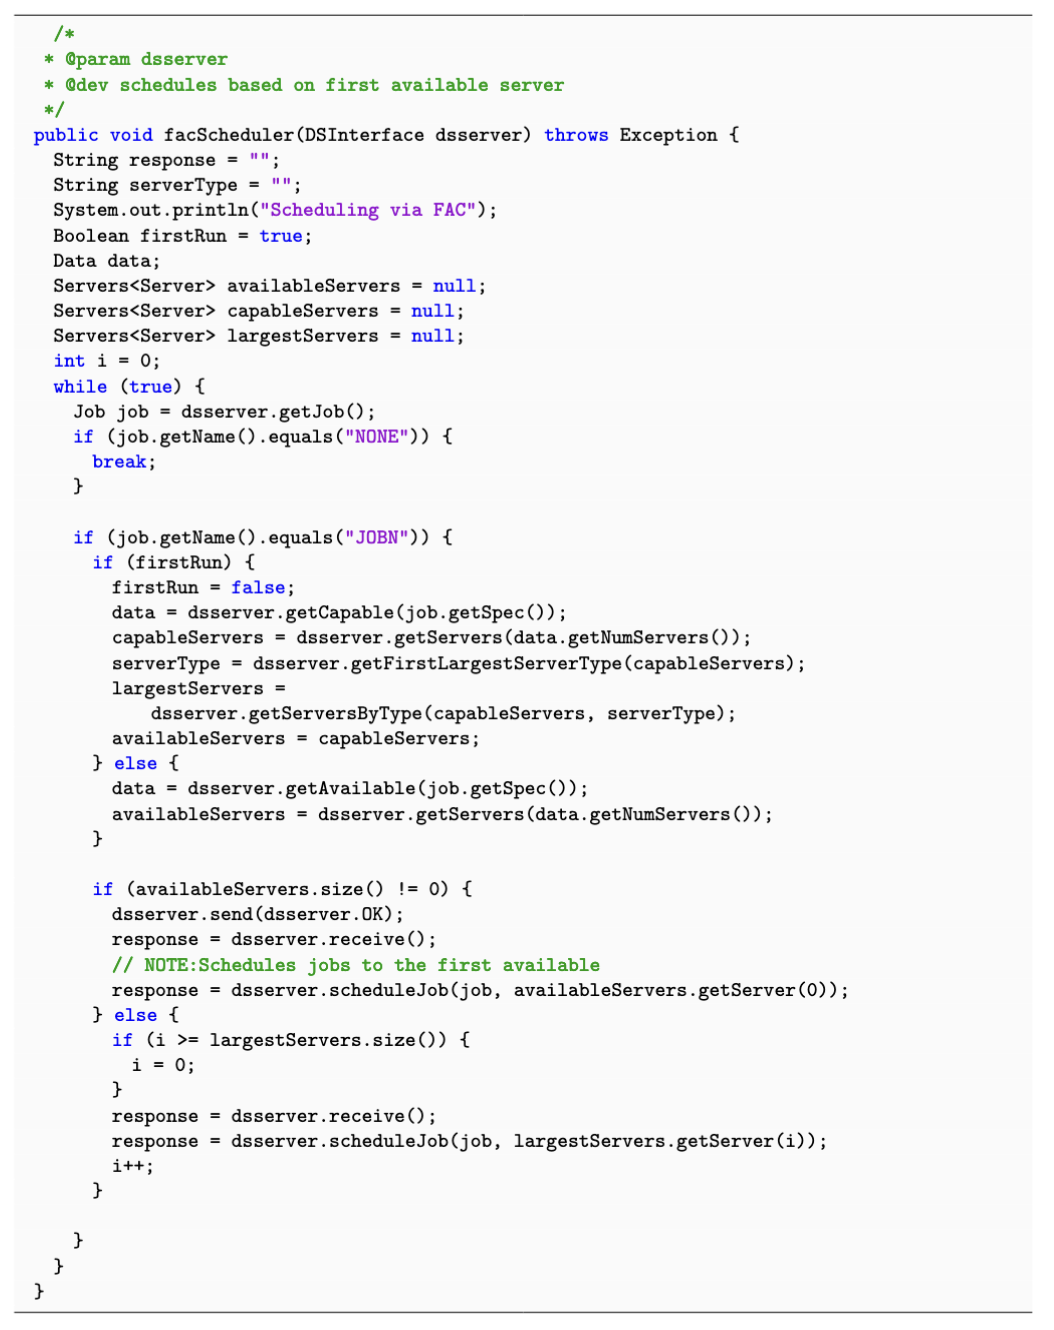
\includegraphics[scale=0.8]{images/code.png}
    \caption{FAC Scheduler Implementation}
    \label{code}
\end{figure}




\section*{6. Evaluation}

By analysing the optimisation trilemma faced by scheduling algorithms, turnaround time, rental cost and resource utilisation we start by analysing the cost of preferring one dimension over another. The FAC is designed to maximise on turnaround time efficiency, with good resource utilisation at the cost of rental cost.

\subsection*{6.1. Cost Benefits Analysis}
\begin{center}
\begin{tabular}{||c c||} 
 \hline
 Cost & Benefit \\ [0.5ex] 
 \hline\hline
  Increased Rental Cost & Turnaround Efficiency \\ [1ex]
 \hline
Increased Rental Cost & Larger Jobs Processed Faster  \\ [1ex]
 \hline
Code Complexity & Optimised Algorithm \\ [1ex]
 \hline
 Slightly Reduced Utilisation & Turnaround Efficiency  \\ [1ex]
 \hline
\end{tabular}
\end{center}

\subsection*{6.2. Results}
The FAC scheduler exhibits turnaround time efficiency \ref{results}
\begin{figure}[H]
    \centering
    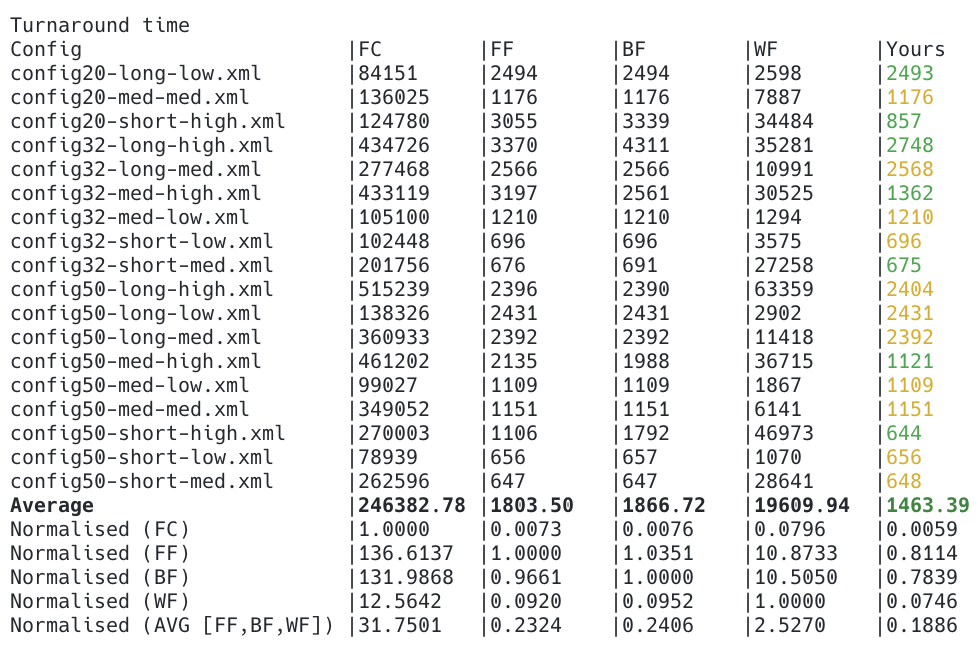
\includegraphics[scale=0.5]{images/turnaround.png}
    \caption{Turnaround Time Results}
    \label{results}
\end{figure}

The FAC scheduler also exhibits moderate utilisation \ref{results}
\begin{figure}[H]
    \centering
    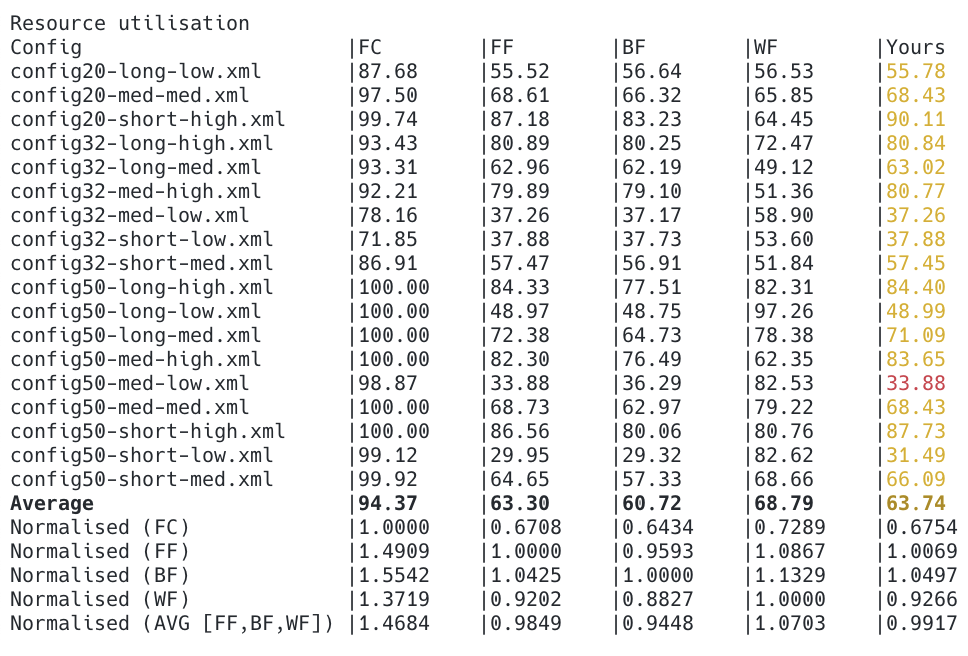
\includegraphics[scale=0.5]{images/utilisation.png}
    \caption{Resource Utilisation Results}
    \label{results}
\end{figure}

The FAC scheduler turnaround time efficiency comes at the detriment to cost \ref{results}
\begin{figure}[H]
    \centering
    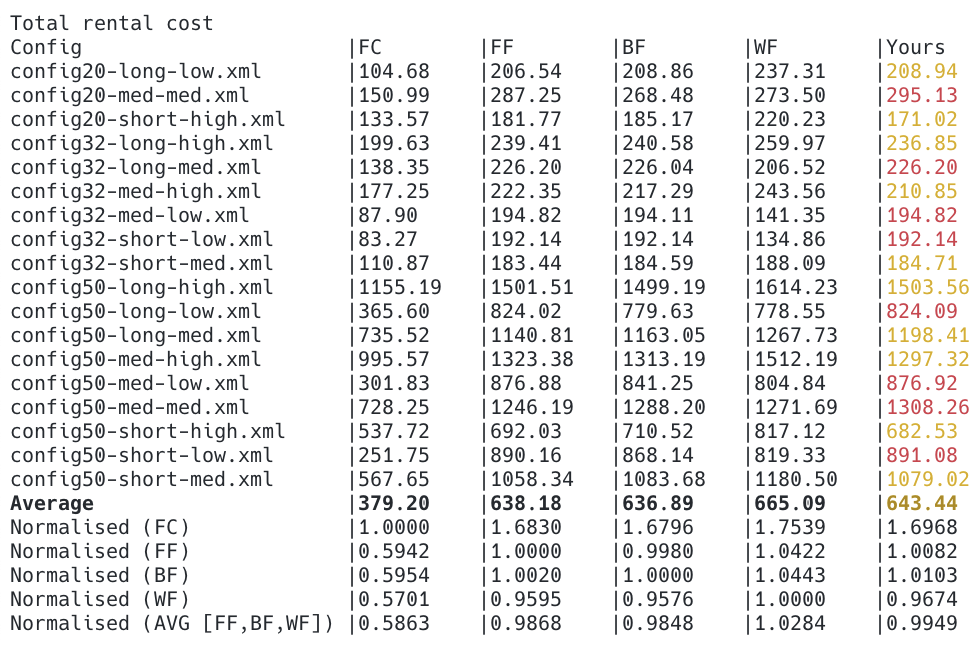
\includegraphics[scale=0.5]{images/cost.png}
    \caption{Rental Cost Results}
    \label{results}
\end{figure}


\section*{Conclusion}
This report has highlighted the inherent tradeoffs involved with designing optimised and efficient algorithms to schedule jobs to servers within a distributed systems environment. We have discussed the trilemma of 1. Turnaround Time 2. Resource Utilisation and 3. Rental Cost. It is clear that there is no one-size-fits-all approach to designing an algorithm. Where potentially there might be optimisations to further improve an algorithm, which may even improve the performance of it on all three basis points, it will still exhibit some performance trade-offs in some basis points as compared to other algorithms. To design an effective algorithm to schedule jobs to the DSSIM server, one must first decide which characteristics they desire from the algorithm. Whether it be effective utilisation of resources, low rental cost or fast turnaround time. 

\subsection*{Source Code Repository}
\begin{itemize}
    \item \hyperlink{https://github.com/beauwilliams/Comp3100}{https://github.com/beauwilliams/Comp3100}
\end{itemize}

%----------------------------------------------------------------------------------------
%	REFERENCE LIST
%----------------------------------------------------------------------------------------
\bibliographystyle{ieeetr}
\bibliography{comp3100project}
% \printbibliography

%----------------------------------------------------------------------------------------

\end{document}
